%
% pda.tex -- Stackautomaten
%
% (c) 2019 Prof Dr Andreas Müller, Hochschule Rapperswil
%
\section{Stackautomaten}
\index{Stackautomat}%
\rhead{Stackautomaten}
Kontextfreie Grammatiken erzeugen Sprachen, die von einem DEA nicht
akzeptiert werden können.
Es ist also eine erweiterte Maschine
nötig, wenn sie solche Sprachen erkennen soll.
Die Erweiterung muss
den DEA mit einem Speicher ausstatten, der zum Beispiel erlaubt, 
in der Sprache $\{0^n1^n\,\;|\; n\in\mathbb N\}$ die Anzahl der
$0$ zu speichern, damit später die Anzahl der $1$
damit verglichen werden kann.

Die einfachste Art von Speicher für diesen Zweck ist ein Stack:
man legt die $0$ auf den Stack, und entfernt für jede $1$ eine 
$0$.
Wenn der Stack am Schluss leer ist, es ``aufgeht'', ist das
Wort akzeptabel.

\subsection{Formale Definition}
\begin{definition}
Ist $\Sigma$ eine endliche Menge, die das leere Wort $\varepsilon$
nicht enthält, dann setzen wir 
\[
\Sigma_\varepsilon = \Sigma\cup \{\varepsilon\}.
\]
\end{definition}

\begin{definition}
\index{Stackautomat}%
\index{Pushdown-Automat|see{Stackautomat}}%
Ein Stackautomat ist ein $6$-Tupel $(Q,\Sigma,\Gamma,\delta,q_0,F)$
mit endlichen Mengen $Q$, $\Sigma$, $\Gamma$ und $F$ und folgenden
Bezeichungen und Einschränkungen
\begin{enumerate}
\index{Zustand}%
\item Die Elemente von $Q$ heissen Zustände.
\index{Eingabe-Alphabet}%
\item $\Sigma$ ist das Eingabe-Alphabet
\index{Stack-Alphabet}%
\item $\Gamma$ ist das Stack-Alphabet
\item $\delta\colon Q\times \Sigma_\varepsilon\times\Gamma_\varepsilon
\to P(Q\times\Gamma_\varepsilon)$ heisst Übergangsfunktion
\index{Startzustand}%
\item $q_0\in Q$ heisst Startzustand
\index{Akzeptierzustand}%
\item $F\subset Q$ heisst Menge der Akzeptierzustände.
\end{enumerate}
\end{definition}
Die Elemente $Q$, $q_0$ und $F$ scheinen für sich genommen
einen endlichen Automaten zu definieren, jedoch einen, der je nach
dem Wert, der als drittes Argument der Übergangsfunktion
übergeben wird, sich etwas anders verhält.
Die Idee ist, dass
dieses dritte Argument von einem Stack gelesen werden soll, der in
der Definition nicht explizit ausgedrückt sein muss, da er
sich für alle Stackautomaten gleich verhält: Man kann Zeichen
aus $\Gamma$ dort hinschreiben, oder von dort lesen\footnote{Man könnte
die Definition eines Stackautomaten auch als C++-Template mit
sechs Template-Argumenten betrachten.
Um den Stack zu
implementieren, muss man nur wissen, was man darauf ablegen will,
man muss also nur $\Gamma$ kennen.}.

Im Gegensatz zu den endlichen Automaten, wo wir grossen Wert auf die
Unterscheidung zwischen deterministischen und nicht deterministischen
Automaten gelegt haben, definieren wir Stackautomaten nur
``nichtdeterministisch''.

\subsection{Gerichteter beschrifteter Graph}
% XXX Idee: Zu den Stack-Operationen Bilder hinzufuegen
\index{Graph!gerichteter!beschrifteter!eines Stackautomaten}%
Auch zu einem Stackautomaten gibt es einen gerichteten beschrifteten
Graphen.
Die Übergangsfunktion legt jetzt zu jedem Zustand 
fest, was für ein Zeichen verarbeitet wird, was für ein
neuer Zustand erreicht wird, und wie sich der Stackinhalt
verändert.
Dazu wird diese zusätzliche Information der Beschriftung der Pfeile
hinzugefügt.
\[
\xymatrix{
*++[o][F]{p}\ar[r]^{a,b\to c}
	&*++[o][F]{q}
}
\]
bedeutet, dass der Automat bei der Verarbeitung eines Zeichens $a$
vom Zustand $p$ in den Zustand $q$ übergeht, wenn gleichzeitig
ein Zeichen $b$ zuoberst auf dem Stack durch das Zeichen $c$
ersetzt werden kann.
Für Übergänge mit dem leeren Wort gilt:
\[
\xymatrix{
*++[o][F]{p}\ar[r]^{a,\varepsilon\to c}
	&*++[o][F]{q}
		&\text{$c$ wird auf den Stack gelegt}
\\
*++[o][F]{p}\ar[r]^{a,b\to\varepsilon}
	&*++[o][F]{q}
		&\text{$b$ wird vom Stack entfernt}
\\
*++[o][F]{p}\ar[r]^{a,\varepsilon\to\varepsilon}
	&*++[o][F]{q}
		&\text{Stack bleibt unverändert}
}
\]
In allen Fällen darf $a$ auch das leere Wort sein, was Operationen
ergibt, die den Stack verändern, ohne dass dazu Input verarbeitet werden
muss.

% XXX weitere Illustrationen der Stack-Operationen hinzufuegen:
% p --- eps,b->eps ---> q
% p --- eps,eps->eps ---> q

\subsection{Beispiele\label{stackbeispiele}}
\subsubsection{Stackautomaten können ``zählen''}
Um die Wörter der nicht reguläre Sprache
$L=\{\texttt{0}^n\texttt{1}^n\;|\;n\in \mathbb N\}$
zu erkennen, braucht man einen Zähler, mit dem man die Zahl der $\texttt{0}$
mit der Zahl der $\texttt{1}$ vergleichen kann.
In einem endlichen Automaten
gab es dafür keinen Platz, aber der Stack eines Stackautomaten kann
diese Aufgabe übernehmen.

Um zu erkennen, dass der Stack wieder leer ist, braucht man ein Zeichen,
welches den Anfang des Stacks markiert.
Das Stack-Alphabet muss also 
etwas grösser sein, wir fügen das Zeichen {\tt \$} hinzu, also
$\Gamma=\{{\tt 0},{\tt 1},{\tt \$}\}$.
Die Idee des konstruierten Stackautomaten ist den Stack als Ablage der
verarbeiteten {\tt 0} zu verwenden, und anschliessend beim verarbeiten
der  {\tt 1} die Nullen wieder vom Stack zu nehmen.
Wenn alles ``aufgeht'',
wurde ein Wort mit gleich vielen Nullen wie Einsen verarbeitet, also 
ein Wort in $L$.
\[
\entrymodifiers={++[o][F]}
\xymatrix{
*+\txt{}\ar[r]
	&{}\ar[r]^{\varepsilon,\varepsilon\to{\tt \$}}
		&{} \ar@(ur,dr)^{{\tt 0},\varepsilon\to{\tt 0}}
		    \ar[d]^{\varepsilon,\varepsilon\to\varepsilon}
\\
*+\txt{}
	&*++[o][F=]{}
		&{}\ar[l]^{\varepsilon,{\tt \$}\to\varepsilon}
		   \ar@(ur,dr)^{{\tt 1},{\tt 0}\to\varepsilon}
}
\]
Damit ist gezeigt, dass die nicht reguläre Sprache $L$ von einem Stackautomaten
akzeptiert wird.

\subsubsection{Die Sprache $L=\{a^ib^jc^k\;|\;i,j,k\in\mathbb N, i=j\vee i=k\}$}
Auch in dieser Sprache muss man die $a$ auf den Stack legen, um sie
zu zählen.
Dann muss man sich nicht deterministisch entscheiden,
ob man auf gleich viele $b$ oder auf gleich viele $c$ testen will,
beides kann man nicht haben, da nach einem Test der Stack wieder leer
ist.
Als Alphabet verwenden wir daher wieder $\Gamma=\{a,b,c,{\tt\$}\}$.
Der Automat muss also zunächst das Zeichen {\tt\$} auf den Stack legen.
Dann beginnt er entweder, die $b$ zu zählen, und die $c$ zu ignorieren,
oder die $b$ zu ignorieren und dann die $c$ zu zählen.
\[
\entrymodifiers={++[o][F]}
\xymatrix{
*+\txt{}
	&*+\txt{}\ar[d]
\\
*+\txt{}
	&{}\ar[d]^{\varepsilon,\varepsilon\to{\tt\$}}
\\
{}\ar@(u,l)_{b,a\to\varepsilon}
  \ar[d]_{\varepsilon,\varepsilon\to\varepsilon}
	&{}\ar@(dl,dr)_{a,\varepsilon\to a}
	   \ar[l]_{\varepsilon,\varepsilon\to\varepsilon}
	   \ar[r]^{\varepsilon,\varepsilon\to\varepsilon}
		&{}\ar@(u,r)^{b,\varepsilon\to\varepsilon}
		   \ar[d]^{\varepsilon,\varepsilon\to\varepsilon}
\\
{}\ar@(l,d)_{c,\varepsilon\to\varepsilon}
  \ar[r]_{\varepsilon,{\tt\$}\to\varepsilon}
	&*++[o][F=]{}
		&\ar@(r,d)^{c,a\to\varepsilon}
		  \ar[l]^{\varepsilon,{\tt\$}\to\varepsilon}
}
\]

\subsection{Äquivalenz von Stackautomaten und CFG\label{sect:aequivalenz-cfg}}
So wie reguläre Ausdrücke und endliche Automaten zur Beschreibung
von regulären Sprachen äquivalent sind, so sind auch kontexfreie Grammatiken
mit Stackautomaten äquivalent:

\begin{satz}
Eine Sprache ist genau dann kontextfrei, wenn sie von einem
Stackautomaten akzeptiert wird.
\end{satz}

Es ist einerseits zu zeigen, dass sich für jede Grammatik ein Stackautomat
finden lässt, der die von der Grammatik erzeugte Sprache akzeptiert.
Andererseits muss auch zu einem beliebigen Stackautomaten eine 
Grammatik gefunden werden, welche die gleiche Sprache erzeugt, die
auch der Stackautomat akzeptiert.

\begin{hilfssatz}\label{hilfssatz_cfg_to_pushdown}
Ist $L$ eine kontextfreie Sprache mit Grammatik $G=(V,\Sigma,R,S)$,
dann gibt es einen Stackautomaten, der $L$ akzeptiert.
\end{hilfssatz}

\begin{proof}[Beweis]
Die Grammatik erzeugt die Wörter dadurch, dass sie auf die Startvariable
immer wieder Regeln aus $R$ anwendet.
Diesen Prozess kann man auf dem
Stack nachbilden.
Zu Beginn legt man die Startvariable auf den Stack.
Die Anwendung von Regeln besteht darin, eine Variable vom Stack zu nehmen,
und stattdessen die Zeichen auf der rechten Seite der Regel
auf den Stack zu legen.

Als Stackalphabet verwenden wir $\Gamma = V\cup \Sigma \cup \{{\tt \$}\}$.
Zu Beginn wird das Symbol {\tt\$} auf den Stack gelegt, am Schluss wird 
es wieder entfernt, es sind also insgesamt vier Zustände erforderlich:
\[
\entrymodifiers={++[o][F]}
\xymatrix{
*+\txt{}\ar[r]
	&{q_0} \ar[r]^{\varepsilon,\varepsilon\to{\tt\$}}
		&{S}\ar[r]^{\varepsilon,\varepsilon\to S}
			&{R}\ar[r]^{\varepsilon,{\tt\$}\to\varepsilon}
				&*++[o][F=]{A}
}
\]
Jetzt müssen im Zustand $R$ noch Übergänge hinzugefügt werden, mit denen
die Regeln abgebildet werden.
Dazu dürfen wir annehmen, dass die Grammatik bereits in Chomsky Normalform
ist.
Wir müssen also nur noch für Regeln der Form $A\to BC$ und $A\to a$
in Übergänge abbilden.
Die Regel $A\to a$ ersetzt die Variable $A$
durch das Terminalsymbol $a$, das erreicht man mit dem Übergang
\[
\entrymodifiers={++[o][F]}
\xymatrix{
{R}\ar@(ur,dr)^{\varepsilon,A\to a}
}
\]
Für die Regel $A\to BC$ brauchen wir einen zusätzlichen Zustand mit
den beiden Übergängen
\[
\entrymodifiers={++[o][F]}
\xymatrix{
R\ar@/^/[r]^{\varepsilon,A\to C}
	&{}\ar@/^/[l]^{\varepsilon,\varepsilon\to B}
}
\]
Sobald auf dem Stack ein Terminalsymbol liegt, kann dieses mit
den Regeln der Grammatik nicht mehr verarbeitet werden, muss 
aber auf das nächste Zeichen des Eingabewortes passen.
Die Regel
\[
\entrymodifiers={++[o][F]}
\xymatrix{
{R}\ar@(ur,dr)^{a,a\to\varepsilon}
}
\]
entfernt ein solches Terminalssymbol, wenn das gleiche Symbol
als Input anliegt.

Schiesslich müssen wir Übergänge für die möglicherweise vorhandene
Regel $S\to\varepsilon$ beschreiben.
Der Übergang 
\[
\entrymodifiers={++[o][F]}
\xymatrix{
{R}\ar@(ur,dr)^{S,S\to\varepsilon}
}
\]
entfernt die Startvariable vom Stack, ohne dass ein Terminalsymbol dort
lieben bleibt.
So kann das leere Wort akzeptiert werden.

Der so konstruierte Automat akzeptiert genau die
Wörter, die von der Grammatik erzeugt werden.
\end{proof}

Wir könnten diesen Beweis mit folgender Notation noch etwas
prägnanter formulieren.
Die Regeln $A\to BC$ werden dadurch abgebildet,
dass ein zusätzlicher Zustand hinzugefügt wird, um in zwei Schritten
die Variable $A$ vom Stack zu entfernen und stattdessen die zwei Variablen
$BC$ dort abzulegen.
Man möchte also eigentlich die Operation $\varepsilon,A\to BC$ implementieren.
Daher soll das Symbol
\[
\entrymodifiers={++[o][F]}
\xymatrix{
{p}\ar[d]^{a,s\to xyz}
\\
{q}
}
\]
implizit zwei neue Zustände $q_1$ und $q_2$ und die zughörigen
Übergänge wie im folgenden Zustandsdiagramm definieren:
\[
\entrymodifiers={++[o][F]}
\xymatrix{
{p}\ar[r]^{a,s\to z}
	&{q_1}\ar[d]^{\varepsilon,\varepsilon\to y}
\\
{q}
	&{q_2}\ar[l]^{\varepsilon,\varepsilon\to x}
}
\]
Analog für beliebige Wörter auf der rechten Seite der Regel,
für ein Wort $w$ der Länge $|w|$ müssen $|w|-1$ neue
Zustände hinzugefügt werden.

\begin{beispiel}[\bf Beispiel]
Für die Grammatik mit den Regeln $S\to {\tt 0}S{\tt 1}\;|\;\varepsilon$
finde man einen Stackautomaten.

Wir haben zwar nur die Übersetzung für Regeln einer Grammatik in
Chomsky Normalform diskutiert, das Prinzip ist jedoch übertragbar.
Wir stellen die Übergänge zusammen, die im Zustand $R$ anzufügen
sind.
Für die Verarbeitung der Terminalsymbole brauchen wir
für jedes Terminalsymbol einen Übergang, der gleichzeitig
ein Symbol vom Input wie vom Stack entfernt:
\begin{equation}
\entrymodifiers={++[o][F]}
\xymatrix{
{R}\ar@(ur,dr)^{{\tt 0},{\tt 0}\to\varepsilon}
   \ar@(ul,dl)_{{\tt 1},{\tt 1}\to\varepsilon}
}
\label{beispiel-tregel}
\end{equation}
Die Regel $S\to\varepsilon$ wird übergeführt in einen Übergang
\begin{equation}
\entrymodifiers={++[o][F]}
\xymatrix{
{R}\ar@(ur,dr)^{\varepsilon, S\to\varepsilon}
}
\label{beispiel-epsilon}
\end{equation}
Die Regel $S\to {\tt 0}S{\tt 1}$ muss übergeführt werden
in die drei Schritte
\begin{equation}
\entrymodifiers={++[o][F]}
\xymatrix{
{R}\ar[rr]^{\varepsilon,S\to{\tt 1}}
	&*+\txt{}
		&{q_1}\ar[dl]^{\varepsilon,\varepsilon\to S}
\\
*+\txt{}
	&{q_2}\ar[ul]^{\varepsilon,\varepsilon\to{\tt 0}}
}
\label{beispiel-0s1regel}
\end{equation}
Jetzt kann man den Ablauf des Akzeptierens des Wortes {\tt 0011}
verfolgen.
Offenbar ist die Ableitung 
\[
S
\overset{\text{(\ref{beispiel-0s1regel})}}{\longrightarrow}
{\tt 0}S{\tt 1}
\overset{\text{(\ref{beispiel-0s1regel})}}{\longrightarrow}
{\tt 00}S{\tt 11}
\overset{\text{(\ref{beispiel-epsilon})}}{\longrightarrow}
{\tt 0011}
\]
Die Tabellen~\ref{beispiel-tabelle} zeigt den Inhalt des 
Input und des Stacks nach jedem Übergang des Stackautomaten.
\begin{table}
\begin{center}
\begin{tabular}{|c|l|c|l|}
\hline
Übergang&Input&Zustand&Stack\\
\hline
                         &{\tt 0011}&$q_0$&\\
                         &{\tt 0011}&$S$  &${\tt \$}$\\
                         &{\tt 0011}&$R$  &$S\quad {\tt \$}$\\
(\ref{beispiel-0s1regel})&{\tt 0011}&$q_1$&${\tt 1}\quad{\tt \$}$\\
(\ref{beispiel-0s1regel})&          &$q_2$&$S\quad {\tt 1}\quad{\tt \$}$\\
(\ref{beispiel-0s1regel})&          &$R$  &${\tt 0}\quad S\quad {\tt 1}\quad{\tt \$}$\\
(\ref{beispiel-tregel})  &{\tt 011} &$R$  &$S\quad {\tt 1}\quad{\tt \$}$\\
(\ref{beispiel-0s1regel})&{\tt 011}&$q_1$&${\tt 1}\quad {\tt 1}\quad{\tt \$}$\\
(\ref{beispiel-0s1regel})&          &$q_2$&$S\quad {\tt 1}\quad {\tt 1}\quad{\tt \$}$\\
(\ref{beispiel-0s1regel})&          &$R$  &${\tt 0}\quad S\quad {\tt 1}\quad {\tt 1}\quad{\tt \$}$\\
(\ref{beispiel-tregel})  &{\tt 11}  &$R$  &$S\quad {\tt 1}\quad {\tt 1}\quad{\tt \$}$\\
(\ref{beispiel-epsilon}) &{\tt 11}  &$R$  &${\tt 1}\quad {\tt 1}\quad{\tt \$}$\\
(\ref{beispiel-tregel})  &{\tt 1}   &$R$  &${\tt 1}\quad{\tt \$}$\\
(\ref{beispiel-tregel})  &{\tt }    &$R$  &${\tt \$}$\\
                         &{\tt }    &$A$  &\\
\hline
\end{tabular}
\end{center}
\caption{Ablauf des Akzeptierens des Wortes {\tt 0011} mit
Hilfe des Stackautomaten zur Grammatik $S\to {\tt 0}S{\tt 1}\;|\;\varepsilon$
\label{beispiel-tabelle}}
\end{table}
\end{beispiel}

\begin{hilfssatz}\label{pda_has_grammar}
Ist $P$ ein Stackautomat, dann gibt es eine Grammatik $G$, die die
gleiche Sprache produziert: $L(P)=L(G)$.
\end{hilfssatz}

\begin{proof}[Beweis]
Wir müssen eine Grammatik konstruieren, die die gleiche Sprache
erzeugt.
Der Stackautomat sollte möglichst nahe an dem in
Hilfssatz \ref{hilfssatz_cfg_to_pushdown} konstruierten liegen, damit es
möglichst einfach wird, sich von der Äquivalenz zu überzeugen.
Wir führen daher an $P$ zunächst drei einfache Modifikationen
durch: 
\begin{enumerate}
\item $P$ hat nur einen einzigen Akzeptierzustand
$q_a$.
Dies erreicht man dadurch, dass man alle Akzeptierzustände über
einen $\varepsilon$-Übergang mit
$q_a$ verbindet, und bisherigen Akzeptierzustände
werden dann zu gewöhnlichen Zuständen degradiert:
\[
\xymatrix{
*++[o][F=]{q}
	&\Rightarrow
		&*++[o][F]{q}\ar[r]^{\varepsilon,\varepsilon\to\varepsilon}
			&*++[o][F=]{q_a}
}		
\]
Der modifizierte Automat akzeptiert die gleichen Wörter wie $P$.
\item Vor dem Akzeptieren wird der Stack geleert.
Dazu wird ein zusätzliches
Zeichen benötigt, welches das Ende des Stacks signalisiert.
Es wird zu
Beginn auf den Stack geschrieben, und als letzter Übergang wieder
vom Stack genommen.
Der Startzustand $q_0$ wird also ersetzt durch einen neuen
Startzustand $q_0'$, mit dem einzigen Übergang 
\[
\entrymodifiers={++[o][F]}
\xymatrix{
*+\txt{}\ar[r]
	&{q_0'}\ar[r]^{\varepsilon,\varepsilon\to {\tt\$}}
		&q_0
}
\]
und der Akzeptierzustand  durch einen neuen Akzeptierzustand $q_a'$ und
den Übergang
\[
\entrymodifiers={++[o][F]}
\xymatrix{
{q_a}\ar[r]^{\varepsilon,{\tt\$}\to\varepsilon}
	&*++[o][F=]{q_a'}
}
\]
\item Jeder Übergang legt ein Zeichen auf den Stack, oder entfernt
eines, aber er macht nicht beides gleichzeitig.
Dazu muss jeder Übergang,
der gleichzeitig ein Zeichen vom Stack nimmt und ein neues dort ablegt,
mit Hilfe eines neuen Zustandes in zwei Übergänge aufgeteilt werden:
\[
\xymatrix{
*++[o][F]{p}\ar[dd]^{a,b\to c}
	&*+\txt{}
		&*++[o][F]{p}\ar[d]^{a,b\to\varepsilon}
\\
	&\Rightarrow
		&*++[o][F]{s}\ar[d]^{\varepsilon,\varepsilon\to c}
\\
*++[o][F]{q}
	&
		&*++[o][F]{q}
}
\]
Ausserdem müssen Übergänge, die gar nicht auf dem Stack operieren,
durch Übergänge ersetzt werden, die ein beliebiges Stacksymbol
schreiben und gleich wieder entfernen:
\[
\xymatrix{
*++[o][F]{p}\ar[dd]^{a,\varepsilon\to \varepsilon}
	&*+\txt{}
		&*++[o][F]{p}\ar[d]^{a,\varepsilon\to x}
\\
	&\Rightarrow
		&*++[o][F]{s}\ar[d]^{\varepsilon,x\to \varepsilon}
\\
*++[o][F]{q}
	&
		&*++[o][F]{q}
}
\]
\end{enumerate}
Damit können wir jetzt zur Konstruktion der Grammatik schreiten.
Die Idee dabei ist, Variablen $A_{pq}$ zu verwenden, die alle 
Wörter erzeugen, die Zustandsübergängen entsprechen,
die den Automaten vom Zustand $p$ in den Zustand $q$ bringen,
und den Stack im gleichen Zustand zurücklassen, den sie vorgefunden
haben.
Wir setzen $A_{pq}$ mit der Menge der Wörter gleich, die
auf diese Weise erzeugt werden können.

Dazu müssen wir verstehen, wie die Wörter entstehen, die von $P$
akzeptiert werden.
Während der Berechnung, die zum Akzeptieren des
Wortes $w$ führt, wird zunächst
irgendein Zeichen $x$ auf den Stack gelegt, und am Ende muss ein
Zeichen entfernt werden, welches $x$ oder auch etwas Anderes sein kann.

Falls das am Ende entfernte Zeichen $x$ ist, können wir dies durch
die Regel $A_{pq}\to aA_{rs}b$ symbolisieren, wobei $a$ das Zeichen
ist, welches zusammen mit dem Ablegen von $x$ vom Input verarbeitet wird,
und $b$ das Zeichen, das mit dem Entfernen von $x$ verarbeitet wird.
Der Stack ist zwischen den Zuständen $r$ und $s$ unverändert, wir
können ihn schematisch wie in Abbildung~\ref{stacknichtleer} darstellen.
\begin{figure}
\begin{center}
%\includegraphics[width=0.85\hsize]{images/stack-2.pdf}
%\includegraphics{images/stack-2.pdf}
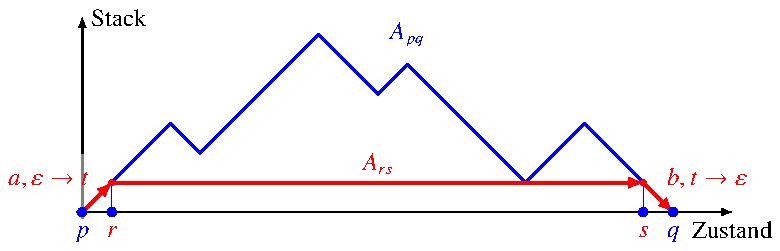
\includegraphics{4-cfg/images/pda-stacknichtleer.pdf}
\end{center}
\caption{Übergänge, die den Stack in keinem Zwischenzustand leeren\label{stacknichtleer}}
\end{figure}

Falls das am Schluss vom Stack entfernte Zeichen nicht das Gleiche ist,
dann muss das $x$ irgendwann im Laufe der Berechnung entfernt worden
sein, und das neue Zeichen $y$ muss auf dem Stack abgelegt worden
sein.
Es gibt also einen Zwischenzustand $r$, in dem der Stack
wieder im selben Zustand wie zu
Beginn der Berechnung ist, wir können dies durch
$A_{pq}\to A_{pr}A_{rq}$ symbolisieren.
Die Abbildung~\ref{stackleer} zeigt diese Situation schematisch.
\begin{figure}
\begin{center}
%\includegraphics[width=0.85\hsize]{images/stack-1.pdf}
%\includegraphics{images/stack-1.pdf}
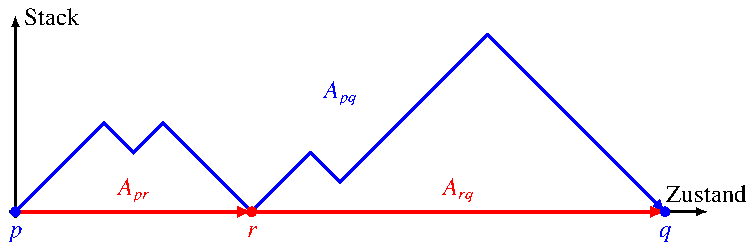
\includegraphics{4-cfg/images/pda-stackleer.pdf}
\end{center}
\caption{Übergänge, die zwischenzeitlich den Stack leeren\label{stackleer}}
\end{figure}

Formal konstruieren wir also eine Grammatik mit Variablen
$V=\{A_{pq}\;|\; p,q\in Q\}$, Startvariable ist $A_{q_0,q_a}$.
Die Menge der Regeln bauen wir wie folgt auf:
\begin{itemize}
\item Für $p,q,r,s\in Q$, $t\in\Gamma$ und $a,b\in\Sigma_{\varepsilon}$:
Falls $\delta(p,a,\varepsilon)$ das Paar $(r,t)$ enthält
und $\delta(s,b,t)$ das Paar $(q,\varepsilon)$, füge die Regel
$A_{pq}\to aA_{rs}b$ hinzu.

Diese Regel besagt, dass Wörter zwischen $p$ und $q$ dadurch gebildet
werden können, dass zunächst ein Zeichen $a$ verarbeitet, und
ein Zeichen $t$ auf den Stack geschrieben wird, dann wird ein Wort
in $A_{rs}$ erzeugt, und zum Schluss das Zeichen $t$ unter
gleichzeitiger Verarbeitung des Zeichens $b$ wieder vom Stack
genommen.

\[
\begin{gathered}
\entrymodifiers={++[o][F]}
\xymatrix{
{p}      \ar[r]^{a,\varepsilon\to t} \ar[d]_{A_{pq}}
	&{r}\ar[d]^{A_{rs}}
\\
{q}
	&{s}\ar[l]^{b,t\to\varepsilon}
}
\end{gathered}
\qquad\rightsquigarrow\qquad A_{pq}\to aA_{rs}b
\]


\item Für drei Zustände $p,q,r\in Q$ füge die Regel 
$A_{pq}\to A_{pr}A_{rq}$ hinzu.
\[
\begin{gathered}
\entrymodifiers={++[o][F]}
\xymatrix{
{p}\ar[dr]^{A_{pr}}\ar[dd]_{A_{pq}}
\\
*+\txt{}
	&{r}\ar[dl]^{A_{rq}}
\\
{q}
}
\end{gathered}
\qquad\rightsquigarrow\qquad A_{pq}\to A_{pr}A_{rq}
\]
\item Für jeden Zustand $p\in Q$ füge die Regel $A_{pp}\to \varepsilon$
hinzu:
\[
\begin{gathered}
\entrymodifiers={++[o][F]}
\xymatrix{
*+\txt{}
	&{p} \ar@(ur,dr)^{A_{pp}}
}
\end{gathered}
\qquad\rightsquigarrow\qquad
A_{pp}\to\varepsilon.
\]
\end{itemize}
Jetzt muss man nur noch zeigen, dass ein Wort $w$ genau dann aus $A_{pq}$
abgeleitet werden kann, wenn es $P$ vom Zustand $p$ mit leerem Stack
in den Zustand $q$ mit leerem Stack bringen kann.


\begin{hilfssatz}\label{apq_generates_x_implies}
Falls $A_{pq}$ das Wort $x$ erzeugt, dann kann $x$ $P$ aus dem Zustand
$p$ mit leerem Stack in den Zustand $q$ mit leerem Stack überführen.
\end{hilfssatz}

\begin{proof}[Beweis von Hilfssatz \ref{apq_generates_x_implies}]
Man kann vollständige Induktion für die Länge der be\-nötigten 
Ableitung $A_{pq}\overset{*}{\Rightarrow} x$ verwenden.

Falls die Ableitung mit nur einem Schritt möglich ist, dann muss
dazu eine Regel der Form $A_{pp}\to\varepsilon$ verwendet werden,
denn dies sind die einzigen Regeln, die auf der rechten Seite
keine Variablen enthalten.

Nehmen wir also an, für Ableitungen der Länge $k$ sei bereits
bekannt, dass sie den Automaten von einem Zustand mit leerem Stack
in einen anderen Zustand mit leerem Stack überführen.

Sei jetzt $A_{pq}\overset{*}{\Rightarrow}x$ eine Ableitung mit $k+1$
Schritten.
Der erste Schritt dieser Ableitung ist entweder eine
Regel der Form $A_{pq}\to aA_{rs}b$ oder $A_{pq}\to A_{pr}A_{rq}$.
Im ersten Fall sagt die Regel, dass $x=ayb$, wobei $y$ ein
Wort ist, welches aus $A_{rs}$ in höchstens $k$ Schritten abgeleitet
werden kann.
Also kann nach Induktionsannahme $y$ den Automaten vom
Zustand $r$ mit leerem Stack in den Zustand $s$ mit leerem Stack
überführen.
Der Übergang von $q$ nach $r$ mit Inputzeichen $a$
legt möglicherweise ein Zeichen $t$ auf den Stack, nach Konstruktion
der Produktionsregeln wird dieses vom Übergang mit Inputzeichen $b$
auch wieder entfernt, so dass der Stack wieder leer ist.

Im zweiten Falls ist nach Induktionsannahme $x=yz$, wobei $y$ den
Automaten vom Zustand $q$ in den Zustand $r$ je mit leerem Stack
überführt, und $z$ ihn von $r$ nach $q$ je mit leerem Stack
führt.

In beiden Fällen folgt, dass $x$ den Automaten von $p$
nach $q$ je mit leerem Stack führen kann.
Damit ist der Induktionsschritt vollzogen, und es folgt, dass
sich jede Ableitung durch Übergänge im Stackautomaten zwischen
Zuständen mit jeweils leerem Stack bilden lassen.
\end{proof}

\begin{hilfssatz}\label{implies_apq_generates_x}
Falls $x$ $P$ aus dem Zustand $p$ mit leerem Stack in den Zustand
$q$ mit leerem Stack überführen kann, dann ist
$A_{pq}\overset{*}{\Rightarrow} x$.
\end{hilfssatz}

\begin{proof}[Beweis von Hilfssatz \ref{implies_apq_generates_x}]
Auch diesen Teil kann man mit vollständiger Induktion beweisen,
diesmal über die Länge der Berechnung.

Die kürzeste mögliche Berechnung hat $0$ Schritte, d.\,h.~sie endet
im gleichen Zustand, in dem sie begonnen hat.
Und tatsächlich enthält die Grammatik die Regel $A_{pp}\to\varepsilon$, 
so dass das leere Wort tatsächlich aus $A_{pp}$ mit leerem
Stack abgeleitet werden kann.

Nehmen wir jetzt an, dass bereits bekannt ist, dass Berechnungen mit
$k$ Schritten, welche $P$ mit dem Input-Wort $w$ vom Zustand $p$
in den Zustand $q$ je mit leerem Stack dazu führen, dass
$A_{pq}\overset{*}{\Rightarrow} x$.

Sei jetzt also eine Berechnung mit Inputwort $x$
mit $k+1$ Schritten gegeben, die $P$ vom Zustand $p$ in den Zustand $q$ 
je mit leerem Stack führt.
Entweder ist der Stack nur ganz zu
Beginn oder ganz am Schluss leer, oder er wird dazwischen einmal
leer.

Im ersten Fall wird ein Symbol $t$ beim ersten Schritt auf den Stack
gelegt, und beim letzten Schritt entfernt.
Es gibt also zwei Zustände
$r$ und $s$ und Übergänge
\[
\entrymodifiers={++[o][F]}
\xymatrix{
p\ar[r]^{a,\varepsilon\to t}
	&r\ar[r]
		&s\ar[r]^{b,t\to\varepsilon}
			&q
}
\]
Die Berechnung, die $P$ von $r$ in $s$ überführt, ist kürzer, und kann
mit leerem Stack durchgeführt werden.
Also ist sie nach Induktionsannahme der Teil $y$ in $x=ayb$ aus
$A_{rs}$ ableitbar.

Im zweiten Fall zerfällt die Berechnung, in der $x$ $P$ von $p$ in
$q$  mit leerem Stack überführt in zwei Teile, die mit Inputwörtern
$y$ und $z$ $p$ in $r$ bzw.~$r$ in $q$ je mit leerem Stack überführen:
\[
\entrymodifiers={++[o][F]}
\xymatrix{
p\ar[r]
	&r\ar[r]
		&q
}
\]
Nach Induktionsannahme ist daher
$A_{pr}\overset{*}{\Rightarrow}y$
$A_{rq}\overset{*}{\Rightarrow}z$, und zusammen mit der Regel
$A_{pq}\to A_{pr}A_{rq}$ der Grammatik auch
$A_{pq}\overset{*}{\Rightarrow} x$
\end{proof}

Damit ist auch der Beweis von Hilfssatz \ref{pda_has_grammar} vollständig.
\end{proof}

\begin{beispiel}
Wir möchten die Theorie dazu verwenden, für den Stackautomaten aus
Abschnitt~\ref{stackbeispiele} für die Sprache
$L=\{\texttt{0}^n\texttt{1}^n\;|\; n\ge 0\}$ eine Grammatik zu finden.
Dazu wandeln wir zunächst den Stackautomaten in die Standardform um, die
wir für die Konstruktion der Grammatik brauchen.
Dazu müssen wir im vertikalen Übergang einen Zwischenzustand einfügen:
\[
\entrymodifiers={++[o][F]}
\xymatrix{
*+\txt{}\ar[r]
	&{q_0}\ar[r]^{\varepsilon,\varepsilon\to{\tt \$}}
		&{q_1} \ar@(ur,dr)^{{\tt 0},\varepsilon\to{\tt 0}}
		    \ar[d]^{\varepsilon,\varepsilon\to x}
\\
*+\txt{}
	&*+\txt{}
		&{q_2}\ar[d]^{\varepsilon,x\to\varepsilon}
\\
*+\txt{}
	&*++[o][F=]{q_a}
		&{q_3}\ar[l]^{\varepsilon,{\tt \$}\to\varepsilon}
		   \ar@(ur,dr)^{{\tt 1},{\tt 0}\to\varepsilon}
}
\]
Die Startvariable der Grammatik ist $A_{q_0q_a}$.
Die Übergänge, die
das Zeichen $\texttt{\$}$ behandeln, führen zu einer Regel
\begin{equation}
A_{q_0q_a}\to \varepsilon A_{q_1q_3}\varepsilon = A_{q_1q_3}.
\label{q0qa}
\end{equation}
Wenn man im Zustand $q_1$ eine $\texttt{0}$ auf den Stack legt, dann
muss man sie auch im Zustand $q_3$ wieder entfernen.
Dieser Prozess gibt Anlass zu einer Regel
\begin{equation}
A_{q_1q_3}\to \texttt{0}\; A_{q_1q_3}\;\texttt{1}
\label{q1q3}
\end{equation}
Man kann aber auch ohne eine $\texttt{0}$ auf dem Stack von
$q_1$ zu $q_3$ gelangen, das führt zu der Regel 
\begin{equation}
A_{q_1q_3}\to \varepsilon\; A_{q_2q_2}\;\varepsilon
\label{q2q2}
\end{equation}
Zusätzlich hat man noch die Regel $A_{q_2q_2}\to\varepsilon$, da 
$A_{q_2q_2}$ nur in (\ref{q2q2}) gebraucht wird, können wir sie
bereits anwenden, und erhalten so die Grammatik.
\begin{align}
A_{q_0q_a}&\to A_{q_1q_3} \tag{\ref{q0qa}}\\
A_{q_1q_3}&\to \texttt{0}\; A_{q_1q_3}\;\texttt{1} \tag{\ref{q1q3}}\\
A_{q_1q_3}&\to \varepsilon\tag{\ref{q2q2}}
\end{align}
Es werden nur noch zwei Variablen verwendet, aber die Startvariable
wird immer in $A_{q_1q_3}$ umgewandelt, man kann sie also auch noch
einsparen.
Schreiben wir $S=A_{q_1q_3}$ bleibt somit als Grammatik
\begin{align}
S&\to \texttt{0}\; S\; \texttt{1}\tag{\ref{q1q3}}\\
S&\to\varepsilon,\tag{\ref{q2q2}}
\end{align}
genau die Grammatik, die wir früher schon für $L$ gefunden haben.
\end{beispiel}

